
\chapter{Numerical methods to simulate resolved atomization}

\section{Introduction}

\textbf{MAKE LINK WITH FINAL PART OF INTRODUCTION WHEN IT IS DONE}

Resolution of two-phase flows requires a suitable description of each phase and a careful treatment of the liquid-gas interface. From a numerical point of view, the multi-scale nature of atomization makes it impossible to use the same methods for resolving atomization accurately and for transporting a developed spray, since the characteristic length scales differ by several orders of magnitude. Consequently, different numerical methodologies must be chosen according to the targeted problem. Furthermore, if multi-physical phenomena, such as evaporation or combustion, are present, the range of possible models to be applied becomes even narrower.

The first step to choose a proper methodology is to identify the type of regime to solve. One possible classification of two-phase regimes can be done depending on the distribution and topology of the interface. In this respect, one can distinguish between separate and disperse phase \citepColor[murrone_numerical_2011]: 


%Suitable modeling strategies are needed to resolve a two-phase flow problem. The strategy chosen will depend on many things, such as the coherence of the liquid phase or the ambient conditions. Hence, the same strategies applied when studying injection at take-off conditions might not be the same than the ones required for relight  altitude relight problems, for example.

%A key challenge in two-phase flows is to resolve the fluid-gas interface and its evolution with space and time so that the atomization process can be properly described. Modeling the interface is not an easy task due to the difference in density and viscosity between both fluids, and several strategies have been developed to solve this issue. The scientific community classifies these models in two big families according to the liquid volume fraction contained within a given control volume. These two families are the \textbf{dense core} and the \textbf{disperse liquid phase} approaches:

%A general classification for two-phase flows systems can be done according to how both phases are separated \citepColor[murrone_numerical_2011], see Fig. :

\begin{itemize}

\item \textbf{Separate phase} flows, also known as dense regime, present a clear definition of the interface and both liquid and gaseous phases can be easily identified (Figure \ref{fig:TPF_droplets_example} left). In such cases, the liquid volume fraction is large and the liquid structures are of the same order, or larger, than the cell size, so the atomization dynamics can be captured by the mesh. Within engines, separate phase is found during primary breakup, as shown by the blue regions of Fig. \ref{fig:atomization_regimes_herrmann}. Numerical methods devoted to resolve separate phase regimes are tackled in this chapter, in $\S$\ref{sec:ch2_eulerian_approaches_dense_regime}. Generally, these methods are restricted to non-reactive problems and the multi-physics coupling with evaporation and combustion is not possible.

\item \textbf{Dispersed phase} regime is found when the liquid volume fraction is small and the liquid structures cannot be capture by the main grid. The liquid phase is composed by individual liquid particles (usually called droplets) whose high number and small size hinders the tracking of the interface (Figure \ref{fig:TPF_droplets_example} right). A developed spray produced as a consequence of secondary atomization is an example of dispersed phase systems, illustrated by the intermediate and dilute regimes of Figure \ref{fig:atomization_regimes_herrmann}. The same numerical methods used for the separate phase regime cannot be applied, since the characteristic scales are much smaller and the grid resolution required yields the computations unaffordable due to their high cost. Numerical formalisms targeting dispersed phase flows are discussed in Chapter \ref{ch3:disperse_phase_methods}. These methods do not resolve atomization as accurately as the ones employed for separate phases, but present the possibility to integrate evaporation and combustion.

\end{itemize}

\begin{figure}[h!]	
	\centering
	\includeinkscape[inkscapelatex=false,scale=0.75]{./part1_numerical_approaches/figures_ch2/TPF_approaches_example}
	\caption{Two-phase systems classification. \textsl{Left}: separate flow, where both phases are easily distinguished and the interface $\Gamma$ can easily be tracked. \textsl{Right}: dispersed phase flow, where individual fluid particles (disperse phase) are surrounded by the gas (carrier phase). In such systems, the interface can hardly be tracked due to the higher surface-to-volume ratio.}
	\label{fig:TPF_droplets_example}
\end{figure}

%Different numerical models have been developed to solve two-phase flows. Due to the differences aforementioned, each method will target problems involving mainly either separate or disperse phase. Volume of fluid ($\S$\ref{subsec:ch2_VOF}) or level-set ($\S$\ref{subsec:ch2_ACLS}) methods are suitable for solving primary atomization, but becomes inefficient when applying it to a cluster of small particles product of secondary atomization. Lagrangian methods, dealt in Chapter \ref{ch3:disperse_phase_methods}, are suitable to represent disperse phase systems containing droplets moving individually, but cannot properly represent a dense liquid region with high volume fraction and would need extra modeling to represent the physics more accurately \citepColor[reitz_modeling_1987].

An \colorbox{red}{insightful} classification of existing numerical methods for two-phase flows is shown in Figure \ref{fig:classification_numerical_methods_mirjalili}. Methods aiming at solving disperse-phase flows use often a two-fluid formulation, since the description of each phase is often done with separate equations. On the other hand, methods addressing separate phases are based on a one-fluid formulation, since basically the same governing equations are solved but distinguishing between phases via their different physical properties. This requires a specific treatment of the interface and the jump conditions in pressure due to surface tension, which each method will handle differently. 

This chapter gives an overview on the state-of-the-art in numerical methods applicable to resolve separate phase regimes. Section \ref{sec:ch2_governing_equations} introduces the governing equations of non-reactive two phase flows, beginning by introducing the Reynolds Transport Theorem and applying it to obtain mass and momentum conservation laws. Section \ref{sec:ch2_eulerian_approaches_dense_regime} presents the numerical methodologies reviewed: diffuse interface, front-tracking, Volume of Fluid (VOF), and Accurate Conservative Level-Set coupled with Ghost-Fluid Method (ACLS/GMF). The last one is the methodology used in this thesis for performing resolved simulation atomizations in Chapter \ref{ch5:jicf_resolved_simulations}.


\begin{figure}[h!]
	\centering
	\includegraphics[scale=1.0]{./part1_numerical_approaches/figures_ch2/classification_numerical_methods_mirjalili}
	\caption{Numerical methods to simulate two-phase flows. Ellipses denote interface-capturing methods. Sharp-interface methods are denoted by a white background, while the grey one indicates diffuse-interface methods. Source: \citeColor[mirjalili_interface-capturing_2017]}
	\label{fig:classification_numerical_methods_mirjalili}
\end{figure}

%Figure \ref{fig:classification_numerical_methods_mirjalili} depicts another classification of methods for two-phase flows according to how they see the interface: \textbf{sharp interface} (white background boxes) and \textbf{diffuse interface} (grey background). The former, as their name indicates, identify the interface as a diffused spatial region where both phases coexists. Diffuse-interface methods are succinctly presented in $\S{subsec:ch2_DI_methods}$. Sharp interface methods, some of which are presented in later sections, see the interface as an infinitely-thin front moving at a certain speed. Hence, the interface is located at a given value of a scalar function which is advected by the fluid. 


\section{Governing equations }
\label{sec:ch2_governing_equations}

\subsection{Reynolds transport theorem}

\subsubsection*{General form}

The starting point for deriving all the conservation equations is the Reynolds transport theorem (RTT). Let's consider a control volume $\Omega$ bounded by a control surface $\partial \Omega$. Let's also consider a control mass $\Omega_m$ which moves with time to enclose the same amount of mass. This control mass coincides at some time instant with the control volume. The RTT relates the variation of a property $\phi = \phi \left( \boldsymbol{x}, t \right)$ in the control mass with its variation in the control volume. In its most general form, it can be expressed as follows \citepColor[collado_reynolds_2007]:

\begin{equation}
\label{eq:RTT_more_general_shape}
\frac{d}{dt} \int_{\Omega_m} \phi  dV =  \frac{ d}{dt} \int_\Omega \phi dV + \int_{\partial \Omega} \phi  \left( \boldsymbol{u} - \boldsymbol{u_c} \right) \cdot \boldsymbol{n}  dS
\end{equation}

where $\boldsymbol{u}$ is the flow velocity at the boundaries, $\boldsymbol{u_c}$ is the velocity of the control surface and $\boldsymbol{n}$ is the normal unit vector pointing outwards the surface of the control volume. Bold symbols indicate vectorial quantities. 

The first term in the right hand side can be expanded by applying Leibniz's integral rule to a domain with moving boundaries. Following the introduced notation, Leibniz's rule takes the following shape:

\begin{equation}
\label{eq:reynolds_transport_theorem_general_controlVolume}
\frac{d}{dt} \int_\Omega \phi dV =  \int_\Omega \frac{\partial \phi}{\partial t} dV + \int_{\partial \Omega} \phi \left( \boldsymbol{u_c} \cdot \boldsymbol{n} \right) dS
\end{equation}

The latter equation can also be seen as another expression for the RTT particularised for a moving control volume. Introducing it into (\ref{eq:RTT_more_general_shape}) yields:


\begin{equation}
\label{eq:reynolds_transport_theorem_general_controlMass}
\boxed{
\frac{d}{dt} \int_{\Omega_m} \phi  dV = \int_\Omega \frac{\partial \phi}{\partial t} dV + \int_{\partial \Omega} \phi   \left( \boldsymbol{u} \cdot \boldsymbol{n} \right) dS
}
\end{equation}

This formulation of the relates the lagrangian formulation of a system (left hand side, corresponding to the control mass) with the eulerian formulation (right hand side, corresponding to the control volume). 

In this document all the control volumes selected for performing balances will be fixed in space, so their boundaries not move. Consequently, $\boldsymbol{u_c} = 0$ and hence Eq. (\ref{eq:reynolds_transport_theorem_general_controlVolume}) becomes $\frac{d}{dt} \int_\Omega \phi dV =  \int_\Omega \partial \phi/\partial t ~ dV$.

\subsubsection*{Application to two-phase flows}
	\label{subsec:RTT_applied_to_TPS_with_interface}

In the particular case of two-phase flows systems comprising gas and liquid phases, denoted respectively by the subscripts $g$ and $l$, the domain can be decomposed into two subdomains $\Omega_\mathrm{g}$ and $\Omega_\mathrm{l}$. The addition of these two subdomains will make the total domain $\Omega$:

\begin{equation}
\label{eq:omega_domain_partition}
\Omega = \Omega_\mathrm{g} \cup \Omega_\mathrm{l}
\end{equation}

The RTT must hold for each subdomain, so Eq. (\ref{eq:reynolds_transport_theorem_general_controlMass}) can be applied to each phase separately

\begin{subequations}
\begin{align}
\frac{d}{dt} \int_{\Omega_{m_\mathrm{g}}} \phi ~ dV &=  \int_{\Omega_\mathrm{g}} \frac{\partial \phi}{\partial t} ~ dV + \int_{\partial \Omega_\mathrm{g}} \phi \left( \boldsymbol{u} \cdot \boldsymbol{n} \right) dS\\
\frac{d}{dt} \int_{\Omega_{m_\mathrm{l}}} \phi ~ dV &=  \int_{\Omega_\mathrm{l}} \frac{\partial \phi}{\partial t} ~ dV + \int_{\partial \Omega_\mathrm{l}} \phi \left( \boldsymbol{u} \cdot \boldsymbol{n} \right) dS
\end{align}
\end{subequations}

The surface integral in the right hand side can be decomposed in two different integrals by considering a common boundary shared by both subdomains: the liquid-gas interface $\Gamma$. This interface can be modified with time. Hence, the control boundary $\partial \Omega$ can be expressed as the addition of the following two subdomains:

\begin{equation}
\label{eq:partial_omega_boundaries_partition}
\partial \Omega = \left( \partial \Omega_\mathrm{g} \backslash \Gamma ~ \right) \cup \left( \partial \Omega_\mathrm{l} \backslash \Gamma ~ \right)
\end{equation}

So the RTT for separate phases can be extended as follows:


\begin{subequations}
\begin{align}
\frac{d}{dt} \int_{\Omega_{m_\mathrm{g}}} \phi ~ dV &=  \int_{\Omega_\mathrm{g}} \frac{\partial \phi}{\partial t} ~ dV + \int_{\partial \Omega_\mathrm{g} \backslash \Gamma} \phi \left( \boldsymbol{u} \cdot \boldsymbol{n} \right) dS + \int_{\Gamma} \phi_\mathrm{g} \left( \boldsymbol{u}_{\scriptsize{\Gamma}} \cdot {\boldsymbol{n}_{\scriptsize{\Gamma}}}_\mathrm{g} \right) dS \\
\frac{d}{dt} \int_{\Omega_{m_\mathrm{l}}} \phi ~ dV &=  \int_{\Omega_\mathrm{l}} \frac{\partial \phi}{\partial t} ~ dV + \int_{\partial \Omega_\mathrm{l} \backslash \Gamma} \phi \left( \boldsymbol{u} \cdot \boldsymbol{n} \right) dS + \int_{\Gamma} \phi_\mathrm{l} \left( \boldsymbol{u}_{\scriptsize{\Gamma}} \cdot {\boldsymbol{n}_{\scriptsize{\Gamma}}}_\mathrm{l} \right) dS
\end{align}
\end{subequations}

where $\boldsymbol{u}_{\scriptsize{\Gamma}}$ is the velocity at the interface and $\boldsymbol{n}_{\scriptsize{\Gamma}}$ is the vector normal to the interface pointing outwards its corresponding phase. As the interface is the same but the outward direction is opposed for each phase, an interface normal vector pointing to the liquid phase can be defined: 

\begin{equation}
\boldsymbol{n}_{\scriptsize{\Gamma}} = {\boldsymbol{n}_{\scriptsize{\Gamma}}}_\mathrm{l} = - {\boldsymbol{n}_{\scriptsize{\Gamma}}}_\mathrm{g}
\end{equation}

Hence, the RTT for each separate phase can be reformulated as:

\begin{subequations}
\label{eq:RTT_general_twoEquations}
\begin{align}
\frac{d}{dt} \int_{\Omega_{m_\mathrm{g}}} \phi ~ dV &=  \int_{\Omega_\mathrm{g}} \frac{\partial \phi}{\partial t} ~ dV + \int_{\partial \Omega_\mathrm{g} \backslash \Gamma} \phi \left( \boldsymbol{u} \cdot \boldsymbol{n} \right) dS - \int_{\Gamma} \phi_\mathrm{g} \left( \boldsymbol{u}_{\scriptsize{\Gamma}} \cdot \boldsymbol{n}_{\scriptsize{\Gamma}} \right) dS \\
\frac{d}{dt} \int_{\Omega_{m_\mathrm{l}}} \phi ~ dV &=  \int_{\Omega_\mathrm{l}} \frac{\partial \phi}{\partial t} ~ dV + \int_{\partial \Omega_\mathrm{l} \backslash \Gamma} \phi \left( \boldsymbol{u} \cdot \boldsymbol{n} \right) dS + \int_{\Gamma} \phi_\mathrm{l} \left( \boldsymbol{u}_{\scriptsize{\Gamma}} \cdot \boldsymbol{n}_{\scriptsize{\Gamma}}\right) dS
\end{align}
\end{subequations}

Finally, a general shape for the RTT in two-phase flows can be obtained by adding Equations (\ref{eq:RTT_general_twoEquations}) and applying (\ref{eq:omega_domain_partition}) and (\ref{eq:partial_omega_boundaries_partition}):

\begin{equation}
\label{eq:RTT_general_bothPhases}
\frac{d}{dt} \int_{\Omega_m} \phi dV =  \int_{\Omega} \frac{\partial \phi}{\partial t}  dV + \int_{\partial \Omega} \phi \left( \boldsymbol{u} \cdot \boldsymbol{n} \right) dS + \int_\mathsmaller{\Gamma} \left( \phi_\mathrm{l} - \phi_\mathrm{g} \right) \left( \boldsymbol{u}_{\scriptsize{\Gamma}} \cdot \boldsymbol{n}_{\scriptsize{\Gamma}} \right) dS
\end{equation}





\subsection{Mass conservation}

\subsubsection*{General forms}

The mass conservation equation for a fluid system is obtained by substituting $\phi = \rho$ in Eq. (\ref{eq:reynolds_transport_theorem_general_controlMass}):

\begin{equation}
\frac{d}{dt} \int_{\Omega_m} \rho  dV =  \int_\Omega \frac{\partial \rho}{\partial t} dV + \int_{\partial \Omega} \rho \boldsymbol{u} \cdot \boldsymbol{n} dS
\end{equation}

By definition, the control mass is a region of the fluid flow whose mass does not change. Hence, the left hand side of the previous expression is $0$ and the \textbf{mass conservation in integral form}, or \textbf{weak form of mass conservation}, is expressed as follows:


\begin{equation}
\label{eq:mass_conservation_general_integral}
\boxed{
\int_\Omega \frac{\partial \rho}{\partial t}   dV + \int_{\partial \Omega} \rho \boldsymbol{u} \cdot \boldsymbol{n} dS = 0
}
\end{equation}

The Gauss theorem can be applied to a vectorial field $\boldsymbol{f}$ to transform a surface integral into a volume integral:

\begin{equation}
\label{eq:gauss_theorem}
\int_{\partial \Omega} \boldsymbol{f} \cdot \boldsymbol{n} dS = \int_\Omega \nabla \boldsymbol{f}  dV
\end{equation}

Applying this theorem considering $\boldsymbol{f} = \rho \boldsymbol{u}$ and substituting into (\ref{eq:mass_conservation_general_integral}) yields the general expression for \textbf{mass conservation in differential form} or \textbf{strong form of mass conservation}:

\begin{equation}
\label{eq:mass_conservation_general_differential}
\boxed{
\frac{\partial \rho}{\partial t} + \nabla \left( \rho \boldsymbol{u} \right) = 0
}
\end{equation}

This equation is also known as the \textbf{continuity equation in conservative form}. The \textbf{non-conservative} form can be obtained by expanding the left-hand side:

\begin{equation}
\frac{\partial \rho}{\partial t} + \nabla \left( \rho \boldsymbol{u} \right) = \frac{\partial \rho}{\partial t} + \boldsymbol{u} \cdot \nabla \rho  + \rho \nabla \boldsymbol{u} = 0 ~~~~ \rightarrow ~~~~ \frac{d \rho}{d t} + \rho \nabla \boldsymbol{u} = 0
\end{equation}

where $d / d t = \partial / \partial t + \boldsymbol{u} \cdot \nabla $ is the \textbf{material derivative}. 

Hereafter, the weak form of mass conservation will be addressed for its application in integral balances.

\subsubsection*{Global mass conservation in two-phase flows}

A global expression for mass conservation can be obtained by substituting $\phi = \rho$ into Eq. (\ref{eq:RTT_general_bothPhases}):

\begin{equation}
\frac{d}{dt} \int_{\Omega_m} \rho dV =   \int_{\Omega}  \frac{\partial \rho}{\partial t}  dV + \int_{\partial \Omega} \rho \boldsymbol{u} \cdot \boldsymbol{n} dS + \int_\mathsmaller{\Gamma} \left( \rho_\mathrm{l} - \rho_\mathrm{g} \right) \left( \boldsymbol{u}_{\scriptsize{\Gamma}} \cdot \boldsymbol{n}_{\scriptsize{\Gamma}} \right) dS
\end{equation}

In conditions where mass exchange takes place, such as the hot environment within combustion chambers, high temperature might produce evaporation of the liquid phase into gaseous phase. In such cases, the left hand side term of the former equation would be a sink term different to zero. However in this work mass exchange is not considered, so this term is zero:

\begin{equation}
\int_{\Omega}  \frac{\partial \rho}{\partial t}  dV + \int_{\partial \Omega} \rho \boldsymbol{u} \cdot \boldsymbol{n} dS + \int_\mathsmaller{\Gamma} \left( \rho_\mathrm{l} - \rho_\mathrm{g} \right) \left( \boldsymbol{u}_{\scriptsize{\Gamma}} \cdot \boldsymbol{n}_{\scriptsize{\Gamma}}\right) dS = 0
\end{equation}

It can be noticed that the first two integrals in this expression correspond to the weak form for mass conservation as given by Eq. (\ref{eq:mass_conservation_general_integral}). Hence, this expression is simplified to:

\begin{equation}
\int_\mathsmaller{\Gamma} \left( \rho_\mathrm{l} - \rho_\mathrm{g} \right) \left( \boldsymbol{u}_{\scriptsize{\Gamma}} \cdot \boldsymbol{n}_{\scriptsize{\Gamma}} \right) dS = 0
\end{equation}

As both $\rho_\mathrm{l}$ and $\rho_\mathrm{g}$ are always positive, and $\rho_\mathrm{l} > \rho_\mathrm{g}$ for most known applications (including gas turbines and atmospheric two-phase systems), the only possibility for this expression to hold true is when the dot product is zero:

\begin{equation}
\label{eq:continuity_TPF_noFluxThroughInterface}
\boxed{
\boldsymbol{u}_{\scriptsize{\Gamma}} \cdot \boldsymbol{n}_{\scriptsize{\Gamma}} = 0
}
\end{equation}

which means that the flow velocity normal to the interface must be zero, i.e. there is no liquid or gas crossing the interface. 

\subsubsection*{Mass conservation in separate phases}
	\label{eq:mass_conservation_separated_phases}

Two-phase flows must ensure mass conservation for each phase. This can be done by applying the RTT as given by Eqs. (\ref{eq:RTT_general_twoEquations}) to the field $\phi = \rho$. However this formulation introduces the need to deal with the liquid-gas interface, which is often changing in time. A more useful formulation can be developed by the strong form given by (\ref{eq:mass_conservation_general_integral}) to each phase separately \citepColor[drew_theory_1999]. For making it properly, it is necessary to introduce before the definition of \textbf{volumetric fraction} for a plase $k$, $\alpha_k$:

\begin{equation}
\alpha_k = \frac{V_k}{V}
\end{equation}

This magnitude determines the quantity of a given fluid $k$ that is contained in a considered volume $V$. By definition, it follows that $\sum_{k=1}^\mathrm{N_{phases}} \alpha_k = 1$  It can be defined for both gas and liquid phases, $\alpha_\mathrm{g}$ and $\alpha_\mathrm{l}$, so then $\alpha_\mathrm{g} + \alpha_\mathrm{l} = 1$.

Once the volumetric fractions for liquid and gas have been defined, the continuity equation (\ref{eq:mass_conservation_general_differential}) can be defined for each phase as follows:

\begin{subequations}
\begin{align}
\frac{\partial \alpha_\mathrm{g} \rho_\mathrm{g} }{\partial t} + \nabla \left( \alpha_\mathrm{g} \rho_\mathrm{g} \boldsymbol{u}_\mathrm{g} \right) &= 0  \\
\frac{\partial \alpha_\mathrm{l} \rho_\mathrm{l} }{\partial t} + \nabla \left( \alpha_\mathrm{l} \rho_\mathrm{l} \boldsymbol{u}_\mathrm{l} \right) &= 0
\end{align}
\end{subequations}

The integral balance can be obtained by integrating both expressions over a fixed control volume $\Omega$ and applying the Gauss theorem to the divergence term:

\begin{subequations}
\label{eq:mass_conservation_general_bothPhases_showingIntegrals}
\begin{align}
\frac{\partial}{\partial t} \int_{\Omega} \alpha_\mathrm{g} \rho_\mathrm{g} dV + \int_{\partial {\Omega}} \alpha_\mathrm{g} \rho_\mathrm{g} \left( \boldsymbol{u}_\mathrm{g} \cdot \boldsymbol{n} \right) dS &= 0  \\
\frac{\partial}{\partial t} \int_{\Omega} \alpha_\mathrm{l} \rho_\mathrm{l} dV + \int_{\partial {\Omega}} \alpha_\mathrm{l} \rho_\mathrm{l} \left( \boldsymbol{u}_\mathrm{l} \cdot \boldsymbol{n} \right) dS &= 0 
\end{align}
\end{subequations}

These equations present two components: a transient term and a surface term. The transient term has an effect when the mass of any phase is growing inside the control volume, e.g. at the first instants of fuel injection, when the fuel mass is increasing with time. Once a steady-state has been reached, this term becomes $0$. The surface term accounts for the mass fluxes that are entering of leaving the system through its boundaries. From this term, the \textbf{mass flow rate} $\dot{m}$ of a flux going though an area $A$ can be defined as:

\begin{equation}
\boxed{
\label{eq:mass_flow_rate_definition_general}
\dot{m} = \int_A \rho \left( \boldsymbol{u} \cdot \boldsymbol{n} \right) dS
}
\end{equation}

An inspection of this equation reveals a dot product between the velocity vector and the normal vector to the surface. As the normal vector is pointing outwards the control volume, the dot product will be positive in surfaces where both vectors have the same direction, and negative otherwise. Hence, the mass flow rate will be positive in outlets and negative in inlets.

If the transient term in (\ref{eq:mass_conservation_general_bothPhases_showingIntegrals}), which is a source term, is denoted as $\dot{\Omega}_m$, then the mass conservation for separated phases can be written as follows:

\begin{subequations}
\begin{align}
\dot{\Omega}_{m_\mathrm{g}} + \sum_i \dot{m}_{g_i} &= 0  \\
\dot{\Omega}_{m_\mathrm{l}} + \sum_j \dot{m}_{l_j} &= 0 
\end{align}
\end{subequations}

Considering that inlet fluxes are negative and outlet fluxes are positive, the equations can be rearranged:

\begin{subequations}
\label{eq:mass_conservation_general_bothPhases_transient}
\begin{empheq}[box=\fbox]{align}
\dot{\Omega}_{m_\mathrm{g}} &= \sum_{i_\mathrm{in}} \dot{m}_{g_i} - \sum_{i_\mathrm{out}} \dot{m}_{g_i}  \\
\dot{\Omega}_{m_\mathrm{l}} &= \sum_{j_\mathrm{in}} \dot{m}_{l_j} - \sum_{j_\mathrm{out}} \dot{m}_{l_j}
\end{empheq}
\end{subequations}

\subsection{Momentum conservation}

\subsubsection*{General forms}

The momentum conservation equation for a fluid system is obtained by substituting $\phi = \rho \boldsymbol{u}$ in Eq. (\ref{eq:reynolds_transport_theorem_general_controlMass}):

\begin{equation}
\frac{d}{dt} \int_{\Omega_m} \rho \boldsymbol{u}  dV =  \int_\Omega \frac{\partial \left( \rho \boldsymbol{u} \right) }{\partial t} dV + \int_{\partial \Omega} \rho \boldsymbol{u} \left( \boldsymbol{u} \cdot \boldsymbol{n} \right) dS
\end{equation}

The left-hand side term represents the ensemble of forces acting in the control mass. These forces can be separated into volume and surface forces. The volume forces will be denoted by $\boldsymbol{b}$; the surface forces include the pressure $p$ and the viscous stress tensor $\overline{\overline{\pmb{\tau}}}$. With this notation, the \textbf{momentum conservation in integral form}, or \textbf{weak form of momentum conservation}, is defined as:

\begin{equation}
\label{eq:momentum_conservation_general_integral}
\boxed{
\int_\Omega \frac{\partial \left( \rho \boldsymbol{u} \right) }{\partial t} dV + \int_{\partial \Omega} \rho \boldsymbol{u} \left( \boldsymbol{u} \cdot \boldsymbol{n} \right) dS =  \int_{\partial \Omega} \left( - p \overline{\overline{\pmb{I}}} + \overline{\overline{\pmb{\tau}}} \right) \boldsymbol{n} dS + \int_\Omega \boldsymbol{b} dV
}
\end{equation}

where $\overline{\overline{\pmb{I}}}$ is the identity matrix. Applying the Gauss theorem (\ref{eq:gauss_theorem}) with $\boldsymbol{f} = \rho \boldsymbol{u} \boldsymbol{u}$ and operating yields the \textbf{momentum conservation in differential form}, or \textbf{strong form of momentum conservation}:

\begin{equation}
\label{eq:momentum_conservation_general_differential}
\boxed{
\frac{\partial \left( \rho \boldsymbol{u} \right) }{\partial t}  + \nabla \left( \rho \boldsymbol{u}  \boldsymbol{u} \right) =  - \nabla p + \nabla \overline{\overline{\pmb{\tau}}} + \boldsymbol{b} 
}
\end{equation}

This solution is also known as the \textbf{conservative form of the momentum equation}. The left-hand side can be further expanded:

\begin{equation}
\frac{\partial \left( \rho \boldsymbol{u} \right) }{\partial t}  + \nabla \left( \rho \boldsymbol{u}  \boldsymbol{u} \right) =  \boldsymbol{u} \underbrace{ \left[ \frac{\partial \rho}{\partial t} +  \nabla \left( \rho \boldsymbol{u} \right) \right]}_{\text{Continuity}\atop\text{equation (\ref{eq:mass_conservation_general_differential})}}  + \rho \left[ \frac{\partial \boldsymbol{u}}{\partial t} +  \boldsymbol{u} \cdot \nabla \boldsymbol{u} \right] = \rho \left( \frac{\partial \boldsymbol{u}}{\partial t} +  \boldsymbol{u} \cdot \nabla \boldsymbol{u} \right) = \rho \frac{d \boldsymbol{u}}{dt}
\end{equation}

%% Intermediate step:
% \rho \frac{\partial \boldsymbol{u}}{\partial t} + \boldsymbol{u} \frac{\partial \rho}{\partial t} + \rho \boldsymbol{u} \nabla \boldsymbol{u} + \boldsymbol{u} \nabla \left( \rho \boldsymbol{u} \right)

With this notation, the \textbf{non-conservative form} is obtained:

\begin{equation}
\rho \frac{d \boldsymbol{u}}{dt} =  - \nabla p + \nabla \overline{\overline{\pmb{\tau}}} +  \boldsymbol{b} 
\end{equation}


\subsubsection*{Global momentum conservation in two-phase flows}

A global expression for momentum conservation can be obtained by substituting $\phi = \rho \boldsymbol{u}$ into Eq. (\ref{eq:RTT_general_bothPhases}):

\begin{equation}
\frac{d}{dt} \int_{\Omega_m} \rho \boldsymbol{u} dV =   \int_{\Omega}  \frac{\partial \rho \boldsymbol{u} }{\partial t}  dV + \int_{\partial \Omega} \rho \boldsymbol{u} \left( \boldsymbol{u} \cdot \boldsymbol{n} \right) dS + \int_\mathsmaller{\Gamma} \left( \rho_\mathrm{l} \boldsymbol{u}_\mathrm{l} - \rho_\mathrm{g} \boldsymbol{u}_\mathrm{g} \right) \left( \boldsymbol{u}_{\scriptsize{\Gamma}} \cdot \boldsymbol{n}_{\scriptsize{\Gamma}} \right) dS
\end{equation}

The left-hand side term can be expressed in the same way as in Eq. (\ref{eq:momentum_conservation_general_integral}) with a slight modification: another addend must be included to account for the interface, as done in $\S$\ref{subsec:RTT_applied_to_TPS_with_interface}. In this way, this term becomes:

\begin{equation}
\frac{d}{dt} \int_{\Omega_m} \rho \boldsymbol{u} dV =  \int_{\partial \Omega} \left( - p \overline{\overline{\pmb{I}}} + \overline{\overline{\pmb{\tau}}} \right) \boldsymbol{n} dS + \int_\Omega \boldsymbol{b} dV + \int_{\Gamma} \left[ - \left( p_\mathrm{l} - p_\mathrm{g} \right) \overline{\overline{\pmb{I}}} + \left( \overline{\overline{\pmb{\tau}}}_\mathrm{l} - \overline{\overline{\pmb{\tau}}}_\mathrm{g}  \right) + \overline{\overline{\pmb{\tau}}}_\sigma  \right] \boldsymbol{n} dS
\end{equation}

In the interface term, a new contribution has been added: surface tension, represented in this equation by the tensor $\overline{\overline{\pmb{\tau}}}_\sigma$. Surface tension only contributes in the interface. These terms can now be introduced in the momentum conservation equation:

\begin{multline}
 \int_{\Omega}  \frac{\partial \rho \boldsymbol{u} }{\partial t}  dV + \int_{\partial \Omega} \rho \boldsymbol{u} \left( \boldsymbol{u} \cdot \boldsymbol{n} \right) dS + \int_\mathsmaller{\Gamma} \left( \rho_\mathrm{l} \boldsymbol{u}_\mathrm{l} - \rho_\mathrm{g} \boldsymbol{u}_\mathrm{g} \right) \left( \boldsymbol{u}_{\scriptsize{\Gamma}} \cdot \boldsymbol{n}_{\scriptsize{\Gamma}} \right) dS = \\ = \int_{\partial \Omega} \left( - p \overline{\overline{\pmb{I}}} + \overline{\overline{\pmb{\tau}}} \right) \boldsymbol{n} dS + \int_\Omega \boldsymbol{b} dV + \int_{\Gamma} \left( - \left( p_\mathrm{l} - p_\mathrm{g} \right) \overline{\overline{\pmb{I}}} + \left( \overline{\overline{\pmb{\tau}}}_\mathrm{l} - \overline{\overline{\pmb{\tau}}}_\mathrm{g}  \right) + \overline{\overline{\pmb{\tau}}}_\sigma  \right) \boldsymbol{n} dS
\end{multline}

Inspecting this equation reveals that the first two terms in both sides make the general integral form of momentum conservation, Eq. (\ref{eq:momentum_conservation_general_integral}). Therefore, the equation can be simplified:

\begin{equation}
\int_\mathsmaller{\Gamma} \left( \rho_\mathrm{l} \boldsymbol{u}_\mathrm{l} - \rho_\mathrm{g} \boldsymbol{u}_\mathrm{g} \right) \left( \boldsymbol{u}_{\scriptsize{\Gamma}} \cdot \boldsymbol{n}_{\scriptsize{\Gamma}} \right) dS =  \int_{\Gamma} \left( - \left( p_\mathrm{l} - p_\mathrm{g} \right) \overline{\overline{\pmb{I}}} + \left( \overline{\overline{\pmb{\tau}}}_\mathrm{l} - \overline{\overline{\pmb{\tau}}}_\mathrm{g}  \right) + \overline{\overline{\pmb{\tau}}}_\sigma  \right) \boldsymbol{n} dS
\end{equation}

By continuity in two phase flow, it was shown that $\boldsymbol{u}_{\scriptsize{\Gamma}} \cdot \boldsymbol{n}_{\scriptsize{\Gamma}} = 0$ in Eq.  (\ref{eq:continuity_TPF_noFluxThroughInterface}). Hence the left hand side is zero:

\begin{equation}
\int_{\Gamma} \left( - \left( p_\mathrm{l} - p_\mathrm{g} \right) \overline{\overline{\pmb{I}}} + \left( \overline{\overline{\pmb{\tau}}}_\mathrm{l} - \overline{\overline{\pmb{\tau}}}_\mathrm{g}  \right) + \overline{\overline{\pmb{\tau}}}_\sigma  \right) \boldsymbol{n} dS = 0
\end{equation}

From this relation, it directly follows that:

\begin{equation}
\boxed{
\left( p_\mathrm{l} - p_\mathrm{g} \right) \overline{\overline{\pmb{I}}} = \left( \overline{\overline{\pmb{\tau}}}_\mathrm{l} - \overline{\overline{\pmb{\tau}}}_\mathrm{g}  \right) + \overline{\overline{\pmb{\tau}}}_\sigma  
}
\end{equation}

As shown by this relation, the effect of surface tension it to introduce a discontinuity in pressure and viscous effects in the interface. 

\subsubsection*{Momentum conservation in separate phases}

Following the same procedure of $\S$\ref{eq:mass_conservation_separated_phases}, the volumetric fraction is used to formulate momentum equations in strong form. Equation (\ref{eq:momentum_conservation_general_differential}) can be applied to each phase for getting separate conservation equations of momentum. However, it must be taken into account that there can be exchange of momentum from one phase to another, something which was not taken into account in the mass equations because it is assumed that there is no mass exchange. This \textbf{momentum exchange} between both phases can be accounted for by adding a source term $\dot{\boldsymbol{s}}$. Then, the strong form of momentum conservation equations for each phase take the following form:

\begin{subequations}
\begin{align}
\frac{\partial \left( \alpha_\mathrm{g} \rho_\mathrm{g} \boldsymbol{u}_\mathrm{g} \right) }{\partial t}  + \nabla \left( \alpha_\mathrm{g} \rho_\mathrm{g} \boldsymbol{u}_\mathrm{g}  \boldsymbol{u}_\mathrm{g} \right) &=  - \nabla \left( \alpha_\mathrm{g} p_\mathrm{g} \right) + \nabla \left( \alpha_\mathrm{g} \overline{\overline{\pmb{\tau}}}_\mathrm{g} \right) + \alpha_\mathrm{g} \boldsymbol{b}_\mathrm{g} + \dot{\boldsymbol{s}}_\mathrm{g} \\
\frac{\partial \left( \alpha_\mathrm{l} \rho_\mathrm{l} \boldsymbol{u}_\mathrm{l} \right) }{\partial t}  + \nabla \left( \alpha_\mathrm{l} \rho_\mathrm{l} \boldsymbol{u}_\mathrm{l}  \boldsymbol{u}_\mathrm{l} \right) &=  - \nabla \left( \alpha_\mathrm{l} p_\mathrm{l} \right) + \nabla \left( \alpha_\mathrm{l} \overline{\overline{\pmb{\tau}}}_\mathrm{l} \right) + \alpha_\mathrm{l} \boldsymbol{b}_\mathrm{l} + \dot{\boldsymbol{s}}_\mathrm{l}
\end{align}
\end{subequations}

The integral balance can be obtained by integrating both expressions over a fixed control volume $\Omega$ and applying the Gauss theorem to the divergence term:

\begin{subequations}
\begin{align}
\frac{\partial}{\partial t} \int_{\Omega} \alpha_\mathrm{g} \rho_\mathrm{g} \boldsymbol{u}_\mathrm{g} dV  + \int_{\partial {\Omega}} \alpha_\mathrm{g} \rho_\mathrm{g} \boldsymbol{u}_\mathrm{g} \left( \boldsymbol{u}_\mathrm{g} \cdot \boldsymbol{n} \right) dS &=  \int_{\partial {\Omega}} \alpha_\mathrm{g} \left( - p_\mathrm{g} \overline{\overline{\pmb{I}}} + \overline{\overline{\pmb{\tau}}}_\mathrm{g} \right) \boldsymbol{n} dS + \int_{\Omega} \alpha_\mathrm{g} \boldsymbol{b}_\mathrm{g} dV + \dot{\boldsymbol{S}}_\mathrm{g} \\
\frac{\partial}{\partial t} \int_{\Omega} \alpha_\mathrm{l} \rho_\mathrm{l} \boldsymbol{u}_\mathrm{l} dV  + \int_{\partial {\Omega}} \alpha_\mathrm{l} \rho_\mathrm{l} \boldsymbol{u}_\mathrm{l} \left( \boldsymbol{u}_\mathrm{l} \cdot \boldsymbol{n} \right) dS &=  \int_{\partial {\Omega}} \alpha_\mathrm{l} \left( - p_\mathrm{l} \overline{\overline{\pmb{I}}} + \overline{\overline{\pmb{\tau}}}_\mathrm{l} \right) \boldsymbol{n} dS + \int_{\Omega} \alpha_\mathrm{l}  \boldsymbol{b}_\mathrm{l} dV + \dot{\boldsymbol{S}}_\mathrm{l}
\end{align}
\end{subequations}

where $\dot{\boldsymbol{S}} = \int_{\partial {\Omega}} \dot{\boldsymbol{s}} dV$. The left hand side of these equations present two terms which are analogue to the ones in the continuity equations (\ref{eq:mass_conservation_general_bothPhases_showingIntegrals}): a transient term accounting for the momentum variation within the control volume and a surface term accounting for the momentum fluxes entering or leaving the control volume through its boundaries. This term defines the \textbf{momentum flow rate}, or \textbf{momentum flux}, $\dot{M}$:

\begin{equation}
\label{eq:momentum_flow_rate_definition_general}
\boxed{
\dot{ \boldsymbol{M} } = \int_A \rho \boldsymbol{u} \left( \boldsymbol{u} \cdot \boldsymbol{n} \right) dS
}
\end{equation}

The right-hand side includes all the contributions from surface and body forces to the change of momentum of the system, plus the source term that will account for the momentum exchange between phases. The surface forces will be all group in the term $\boldsymbol{F}_s$, while the body forces will be denoted as $\boldsymbol{F}_b$. If the transient term of the left-hand side is called $\dot{\boldsymbol{J}}$ and the momentum fluxes are separated into inlet and outlet fluxes, then the momentum conservation for separated phases can be written as follows:

\begin{subequations}
\label{eq:momentum_conservation_general_bothPhases_transient}
\begin{empheq}[box=\fbox]{align}
\dot{\boldsymbol{J}}_{m_\mathrm{g}} &= \sum_{i_\mathrm{in}} \dot{\boldsymbol{M}}_{g_i} - \sum_{i_\mathrm{out}} \dot{\boldsymbol{M}}_{g_i} + \boldsymbol{F}_{s_\mathrm{g}} + \boldsymbol{F}_{b_\mathrm{g}} + \dot{\boldsymbol{S}}_\mathrm{g}  \\
\dot{\boldsymbol{J}}_{m_\mathrm{l}} &= \sum_{j_\mathrm{in}} \dot{\boldsymbol{M}}_{l_j} - \sum_{j_\mathrm{out}} \dot{\boldsymbol{M}}_{l_j} + \boldsymbol{F}_{s_\mathrm{l}} + \boldsymbol{F}_{b_\mathrm{l}} + \dot{\boldsymbol{S}}_\mathrm{l}
\end{empheq}
\end{subequations}

\section{Eulerian approaches for dense regime}
\label{sec:ch2_eulerian_approaches_dense_regime}

Previously, the governing laws for fluid dynamics have been stated in their weak and strong forms. They have been extended to two-phase flows by introducing the volume fraction into the equations and by distinguishing between phases. It has been proved that surface tension introduces a discontinuity in the momentum equation, something the numerical method must deals with. This section presents several interface-capturing methods represented in Fig. \ref{fig:classification_numerical_methods_mirjalili} widely used to solve two-phase flow systems. 


\subsection{Diffuse interface methods}
\label{subsec:ch2_DI_methods}

Diffuse interface is not formerly a method, but a family of them. The interface is not found at a precise spatial location, but is distributed along a transition region where both phases coexist. The liquid fraction of gas and liquid phases must add to 1: $\alpha_l + \alpha_g = 1$. Figure \ref{fig:DI_vs_VOF} shows a droplet solved with a diffuse interface method and a sharp interface (VOF) in the same grid, \colorbox{red}{demonstrating clearly how the interface definition is straightforward in the latter but not so easily to track in the former}.

\begin{figure}[h!]
	\centering
	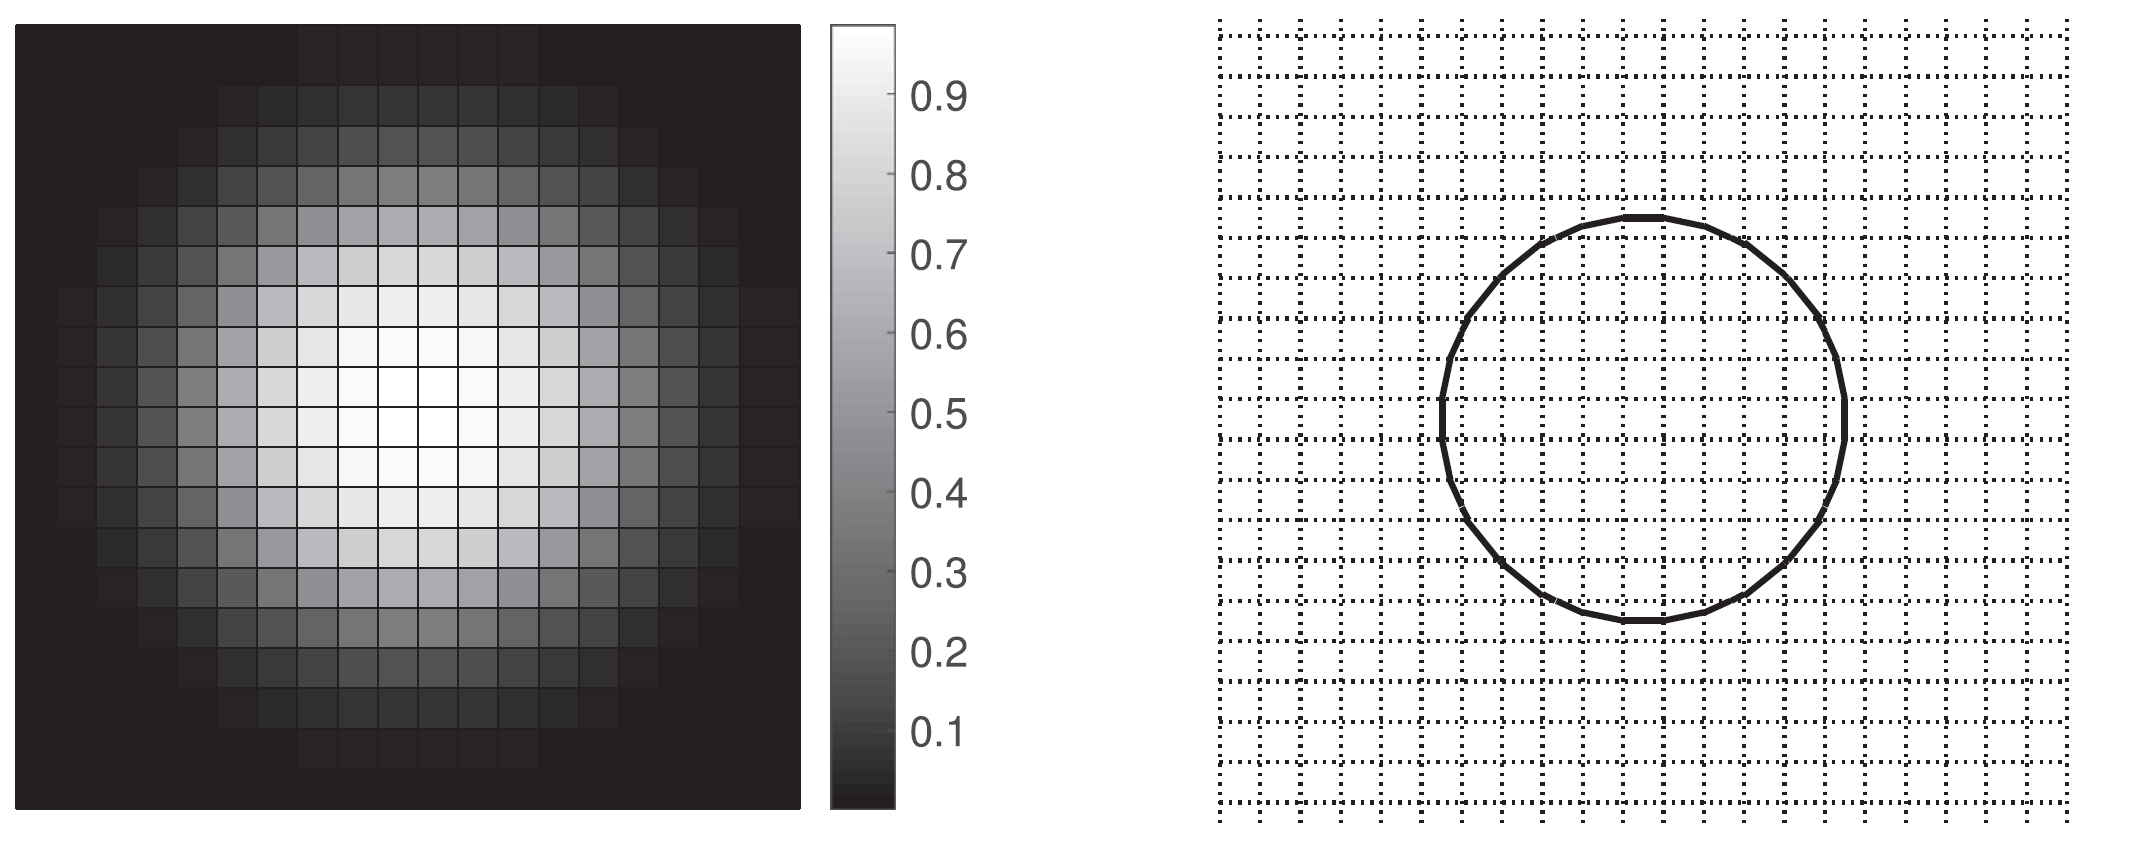
\includegraphics[scale=0.35]{./part1_numerical_approaches/figures_ch2/DI_vs_VOF_Mirjalili}
	\caption{Comparison of a droplet solved in a 20x20 grid by a diffuse interface method (\textit{left}) and a sharp-interface VOF method (\textit{right}). Source: \citeColor[mirjalili_comparison_2019]}
	\label{fig:DI_vs_VOF}
\end{figure}


A class of diffuse-interface methods arousing recent interest in immiscible, incompressible two-phase flows are the phase field methods. Originally, they make use of the Cahn-Hilliard equations \citepColor[cahn_free_1958]. Their derivation is based on the minimisation of a free energy functional, which leads to a typical convection-diffusion equation with source terms. This equation presents the main disadvantage that it is written in a non-conservative form, and hence it is not suitable for its application in immiscible flows \citepColor[mirjalili_conservative_2020]. This issue was later solved by \citeColor[chiu_conservative_2011], who claimed that the following second order equation can be used with the same purpose and applied to immiscible flows:

\begin{equation}
\frac{\partial \psi}{\partial t} + \nabla \left( \textbf{u}  \psi \right) = \nabla \left[ \gamma \left( \epsilon \nabla \psi - \psi \left( 1 - \psi \right) \frac{\nabla \psi}{| \nabla \psi |} \right) \right]
\end{equation}

where $\epsilon$ is a parameter defining the thickness of the interface, $\gamma = \max \left( \textbf{u} \right)$  and $\psi$ is a hyperbolic tangent function representing the distance from the interface, defined later in Eq. (\ref{eq:ACLS_psi_definition}). This equation is transported to obtain the evolution of the interface with time. Then, the velocity fields are obtained from the traditional Navier-Stokes equations with a one-fluid formulation, Eq. (\ref{eq:momentum_conservation_general_differential}). The density and viscosities are evaluated with the field function $\psi$:

\begin{subequations}
\begin{align}
\rho &= \psi \rho_l - \left( 1 -  \psi \right) \rho_g  \\
\mu &= \psi \mu_l   - \left( 1 -  \psi \right) \mu_l
\end{align}
\end{subequations}

Other available diffuse-interface methods have made use of the aforementioned Cahn-Hilliard and applied it to miscible flows \citepColor[teigen_diffuse-interface_2011] and to compressible two-phase systems \citepColor[shukla_interface_2010]. Furthermore, diffuse-interface methods find good applicability in particular thermodynamic regimes, such as multicomponent systems at supercritical conditions where surface tension is non-existent and a proper interface is not present \citemColor[dahms_transition_2013,jofre_transcritical_2021]. 




\subsection{Front-tracking method}

The front-tracking method is, according to the classification of Figure \ref{fig:classification_numerical_methods_mirjalili}, the only method presented in this chapter following an interface-tracking approach (the rest are comprised within the interface-capturing family). It was introduced for the first time by \citeColor[tryggvason_front-tracking_2001]. The interface is modeled as a moving front of lagrangian particles without mass which are explicitly tracked by connected marker points. Particles are convected with the flow field, and their movement is governed according to the kinematic equation:

\begin{equation}
\textbf{u} = \frac{d \textbf{x}}{d t}
\end{equation}

where the velocity $\textbf{u}$ is obtained by solving the flow field. As lagrangian particles are used, the interface is not solved in the same grid as the liquid and gas fields, see Fig. \ref{front_tracking_tryggvason}. This makes this method more of a lagrangian nature than an eulerian one in the sense that the interface is resolved separately from the main grid. Yet, both phases are solved with an eulerian formalisms within the same grid, making this method eulerian since it aims mainly at solving  separate-phase problems as indicated in Fig. \ref{fig:TPF_droplets_example} left. There are indeed interface-tracking methods dealing with the interface from an eulerian perspective, such as the Marker and Cell (MAC) method \citepColor[mckee_mac_2008].

\begin{figure}[h!]
	\centering
	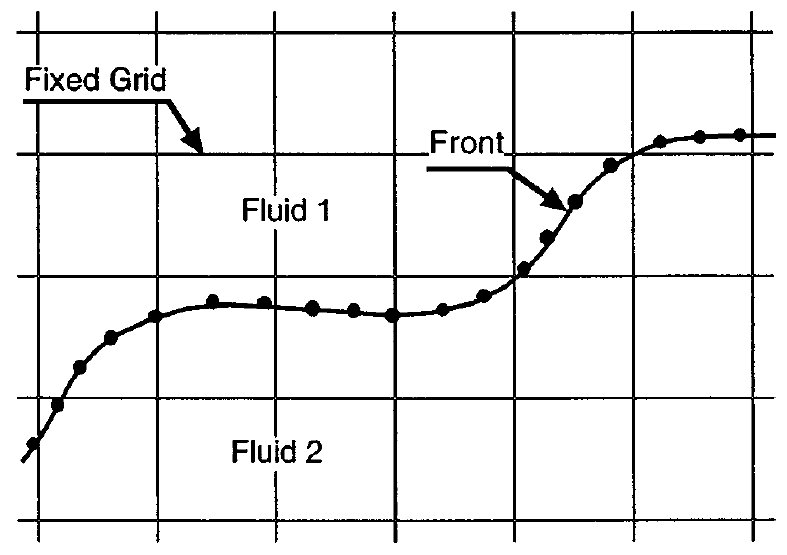
\includegraphics[scale=0.5]{./part1_numerical_approaches/figures_ch2/front-tracking_triggvason}
	\caption{Illustration of the front-tracking method: both fluids are solved in the main grid while the interface is represented by a front of particles. Source: \citeColor[tryggvason_front-tracking_2001]}
	\label{fig:front_tracking_tryggvason}
\end{figure}



\subsection{Volume of Fluid method}
\label{subsec:ch2_VOF}

% VOF reference: 2C. Hirth and B. Nichols. “Volume of Fluid (VOF) method for the dynamics of free boundaries”. In: Journal of Computational Physics 39 (1979), pp. 201–225

The Volume of Fluid method (VOF) is the first numerical methodologies developed to solve for liquid-gas interfaces in free surface flows, introduced originally by \citeColor[hirt_volume_1981]. It is included among the methods using a \textbf{sharp-interface} approach, as opposed to diffuse interface which were succinctly discussed in the previous section. They have been extensively studied in literature , and have been applied for both structured \citemColor[scardovelli_direct_1999,fuster_simulation_2009] and unstructured \citemColor[jofre_3-d_2014,ivey_conservative_2017] grids. VOF methods identify the liquid regions according to their liquid volume fraction $\alpha_l$ defined in Eq.(\ref{eq:volume_fraction_definition}). The volume fraction scalar is transported with an advection equation:

\begin{equation}
	\label{eq:VOF_alpha_advection}
	\frac{\partial \alpha_l}{\partial t} + \nabla \cdot \left( \alpha_l \boldsymbol{u} \right) = 0
\end{equation}

The material properties, density $\rho$ and viscosity $\mu$, are calculated from the liquid volume fraction:

\begin{subequations}
\begin{align}
\rho = \alpha_l \rho_l + \left( 1 - \alpha_l \right) \rho_g  \\
\mu = \alpha_l \rho_l + \left( 1 - \alpha_l \right) \rho_g
\end{align}
\end{subequations}


The biggest advantage of VOF is the mass conservation, as it is ensured when solving \ref{eq:VOF_alpha_advection}. On the other side, its main challenge if the difficulty of reconstructing the interface from the transported $\alpha_\mathrm{l}$ field, as illustrated in Figure \ref{fig:VOF_illustration_drawback}. According to the approach used to reconstruct the interface, VOF methods can be classified as algebraic or geometric \citemColor[mirjalili_interface-capturing_2017,pirozzoli_algebraic_2019].


\begin{figure}[h!]
	\centering
	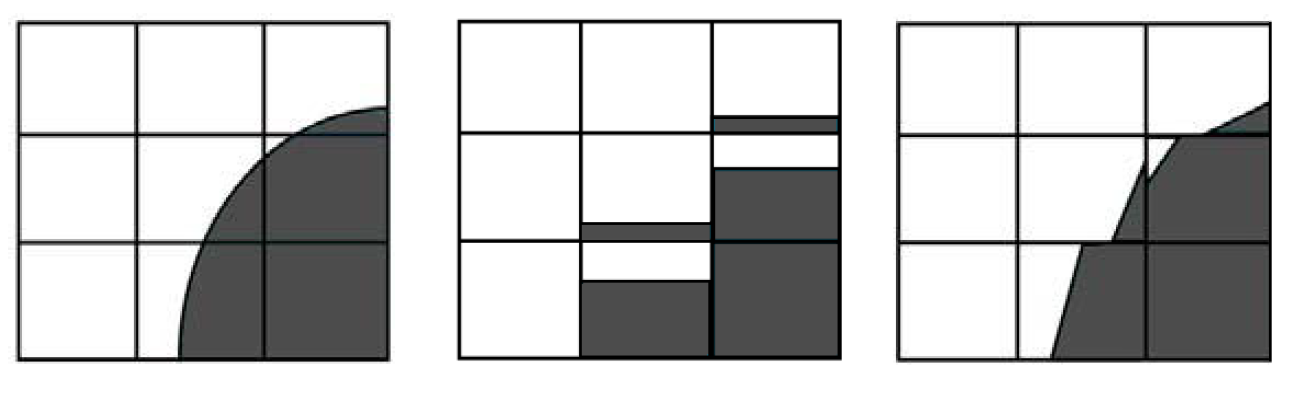
\includegraphics[scale=0.5]{./part1_numerical_approaches/figures_ch2/VOF}
	\caption{Application of VOF method, where dark is liquid and white is gas. \textsl{Left}: original $\alpha_\mathrm{l}$ field. \textsl{Middle}: transported $\alpha_\mathrm{l}$ field. \textsl{Right}: interface reconstruction, where a non-smooth interface can be appreciated. Source: \citeColor[odier_simulation_2006]}
	\label{fig:VOF_illustration_drawback}
\end{figure}


\subsection{Accurate Conservative Level Set method}
\label{subsec:ch2_ACLS}

% Osher and Fedkiw: https://link.springer.com/book/10.1007/b98879
% sussman: https://www.sciencedirect.com/science/article/pii/S0021999184711557
% Olsson articles:
%   https://www.ljll.math.upmc.fr/~hecht/ftp/Mireille-Haddad/A%20conservative%20level%20set%20method%20for%20two%20phase%20flow__Olsson_Kreiss.pdf
%   https://www.ljll.math.upmc.fr/~hecht/ftp/Mireille-Haddad/A%20conservative%20level%20set%20method%20for%20two%20phase%20flow%20II__Olsson.pdf


A well-known class of interface-capturing approaches for two-phase flows are the level set methods. As their own name indicates, these methods identify the interface as a constant value of a scalar level set function. The interface is directly represented and transported using this function, hence its location is always known and no reconstruction needs to be done (as opposed to VOF methods).

Classical level set methods \citepColor[osher_level_2003] distinguish between liquid and gaseous phases by introducing the smooth, signed-distance function to the interface $\phi(\textbf{x},t)$ :

\begin{equation}
\phi \left( \textbf{x},t \right)=\pm |\textbf{x}\left( t \right)-\textbf{x}_{\scriptsize{\Gamma}} \left( t \right)|
\end{equation}

According to this definition, the interface is located at $\phi(\textbf{x},t) = 0$. Positive values of $\phi(\textbf{x},t)$ indicate liquid regions, while negative values denote gas. The interface is then transported with an advection equation:

\begin{equation}
	\label{eq:LS_classical_advection}
	\frac{\partial \phi}{\partial t} + \nabla \cdot \left( \phi \boldsymbol{u} \right) = 0
\end{equation}

When applying the previous expression, the function $\phi$ will be distorted and its smoothness will be lost. To solvent this, the profile of $\phi$ is reshaped using a reinitialization equation \citepColor[sussman_level_1994] However, mass conservation is not ensured after the reinitialization process due to the nature of the distance function $\phi$. In this sense, \citeColor[olsson_conservative_2005] tried to reduce the conservation errors by introducing the hyperbolic tangent function $\psi$:

\begin{equation}
\label{eq:ACLS_psi_definition}
\psi \left( \textbf{x},t \right)=\frac{1}{2} \left(\tanh\left(\frac{\phi(\textbf{x},t)}{2\varepsilon}\right)+1\right)
\end{equation}

where $\varepsilon$ defines the interface thickness. The function $\psi$, which is a mapping from the classical signed-distance $\phi$, is bounded between $0$ and $1$, while $\phi$ is unbounded. The interface $\Gamma$ is located at the iso-value $\psi = 0.5$; gas phase is given by $\psi < 0.5$, and liquid for $\psi > 0.5$. Figure \ref{fig:psi_phi_profiles_janodet_2021_JCP} shows a representative view of both distance functions.

As in the classical level-set method, the hyperbolic tangent profile is also transported via an advection equation:

\begin{equation}
    \frac{\partial \psi}{\partial t} + \boldsymbol{\nabla} \cdot \left( \psi \textbf{u} \right) = 0
\end{equation}

and then reinitialised through resolution of the following equation \citepColor[olsson_conservative_2007]:


\begin{equation}
\label{eq:acls_reinit_2008}
\frac{\partial\psi}{\partial \tau}=\boldsymbol{\nabla}\cdot(\ \underbrace{\varepsilon(\boldsymbol{\nabla}\psi\cdot\textbf{n})\textbf{n}}_{\mathrm{Diffusion}}-\underbrace{\psi(1-\psi)\textbf{n}}_{\mathrm{Resharpening}})
\end{equation}

where $\tau$ is a pseudo-time and $\textbf{n}$ is the normal vector to the interface, obtained from the signed-distance function $\psi$:

\begin{equation}
\textbf{n} = \frac{\nabla \psi}{| \nabla \psi |} 
\end{equation}


As indicated in Eq. (\ref{eq:acls_reinit_2008}), the reinitialization process has two terms: diffusion and resharpening. Both of them are necessary to ensure the smoothness of $\psi$. With the introduction of $\psi$ and the reinitialization equation, mass conservation errors are reduced: hence, this method is referred as conservative level set. Nevertheless, numerical errors might appear during reinitialisation since small oscillations in $\psi$ might induce big variations in $\textbf{n}$. To improve the accuracy, \citeColor[desjardins_accurate_2008] proposed an extension to this conservative methodology in which the interface transport is solved with high order schemes and a fast-marching method is used to reconstruct the signed-distance function $\phi$. This function is then used to compute the interface normals and, with it, the curvature $\kappa$: 

\begin{equation}
\textbf{n} = \frac{\nabla \phi}{| \nabla \phi |} 
\end{equation}

\begin{equation}
\kappa = - \nabla \cdot \textbf{n}
\end{equation}

\citeColor[desjardins_accurate_2008] use a least squares reconstruction to compute $\kappa$. This extension to the conservative level set methodology is known as \textbf{Accurate Conservative Level Set} (ACLS) method. With these formulations, mass conservation is improved and numerical errors are reduced. ACLS is coupled to the Ghost-Fluid Method (GFM) \citepColor[fedkiw_non-oscillatory_1999] in order to deal explicitly with the pressure jump at the interface:

\begin{equation}
    \left[ p \right]_{\scriptsize{\Gamma}} = p_{l,{\scriptsize{\Gamma}}} - p_{g,{\scriptsize{\Gamma}}}  = \sigma \kappa_{\scriptsize{\Gamma}} + 2 \left[ \mu \right]_{\scriptsize{\Gamma}} \textbf{n}^T \cdot \nabla \textbf{u} \cdot \textbf{n}
\end{equation}

where $\kappa_\Gamma$ is the interface mean curvature and $\mu$ is the dynamic viscosity. Using this formulation, surface tension forces $\sigma\kappa_\Gamma$ are embedded in the pressure jump. \\

\begin{figure}[ht]
    \centering
    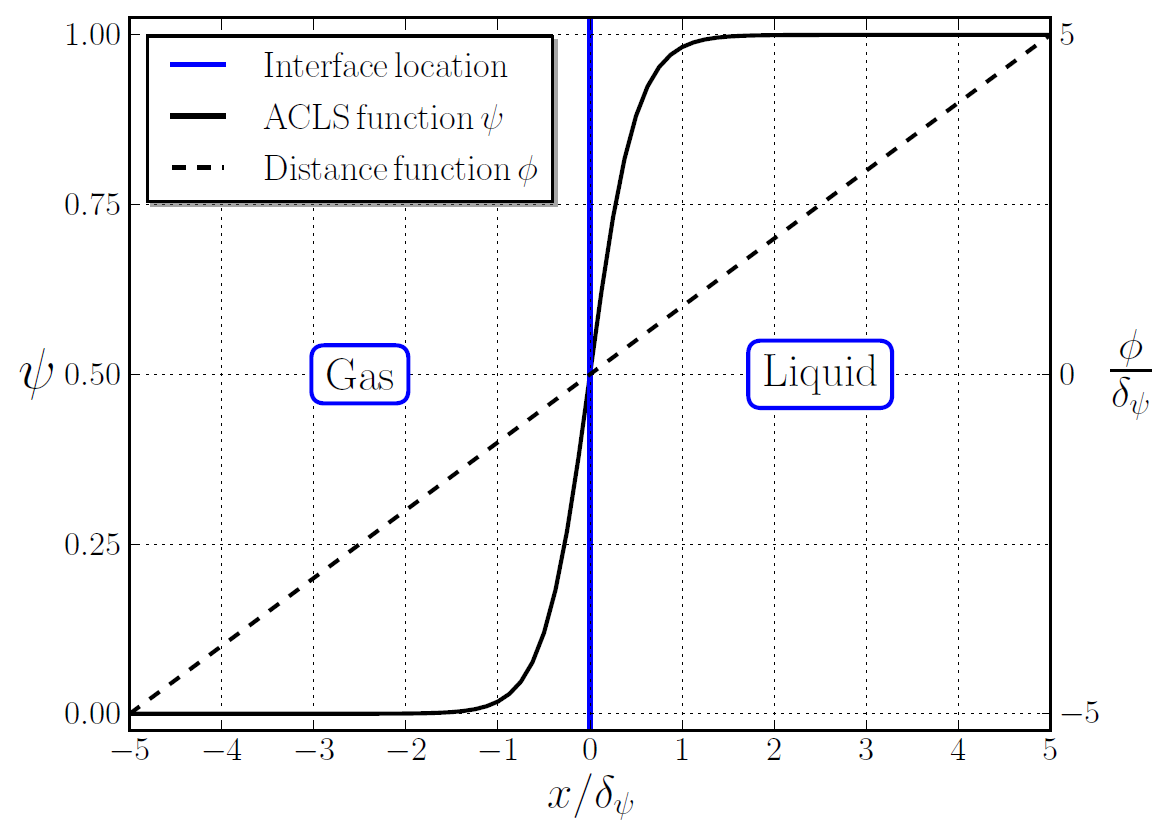
\includegraphics[width=0.6\textwidth]{./part1_numerical_approaches/figures_ch2/ACLS_psi_phi_janodet_JCP}
       \centering
    \caption{Representation of distance functions $\phi$ and $\psi$. The signed-distance function $\phi$ has been normalized by $\delta_\psi = 4\varepsilon$ for visualization. Source: \textbf{ref:Janodet-2021-JCP}.}
    \label{fig:psi_phi_profiles_janodet_2021_JCP}
\end{figure}



In this work, the more recent extension to the ACLS method by \textbf{ref:Janodet-2021-JCP} is used. This formulation makes use of the reinitialization equation introduced by \citeColor[chiodi_reformulation_2017]:

\begin{equation}
\label{eq:acls_reinit_2017}
\frac{\partial\psi}{\partial \tau}=\boldsymbol{\nabla}\cdot\left(\frac{1}{4\cosh^2{\left(\phi_{\mathrm{map}}/2\varepsilon\right)}}\left(|\boldsymbol{\nabla}\phi_{\mathrm{map}}\cdot\textbf{n}|-1\right)\textbf{n}\right)
\end{equation}

where $\phi_{\mathrm{map}}=\varepsilon\ln\left({\psi}/({1-\psi})\right)$ is an analytical signed-distance function mapped for $\psi \in ]0;1[$. This reinitialization equation ensures that the hyperbolic tangent profile $\psi$ is reshaped after transport without introducing significant spurious displacement of the interface. The curvature is then calculated as follows:

\begin{equation}
\kappa=\frac{\mathrm{Tr}\left(\boldsymbol{\mathcal{H}}(\phi)\right)-\frac{\boldsymbol{\nabla}\phi^T}{|\boldsymbol{\nabla}\phi|}\cdot\boldsymbol{\mathcal{H}}\left(\phi\right)\cdot\frac{\boldsymbol{\nabla}\phi}{|\boldsymbol{\nabla}\phi|}}{|\boldsymbol{\nabla}\phi|}
\label{eq:curvature_Goldman}
\end{equation}

where $\mathcal{H} \left( \phi \right)$ is the Hessian matrix of the distance function. To reduce numerical errors, a Geometric-Projection Marker Method (GPMM) is used reconstruct $\phi$ at the nodes in a narrow band around the interface \citepColor[janodet_unstructured_2019]. The GFM method is also used to deal with the interface pressure jump. Both phases are solved with a one-fluid formulation by solving Navier-Stokes and evaluating the physical properties at each spatial location with:

\begin{subequations}
\begin{align}
\rho(\textbf{x},t) &= \rho_g+(\rho_l-\rho_g)H(\psi(\textbf{x},t)-1/2)  \\
\mu(\textbf{x},t) &= \mu_g+(\mu_l-\mu_g)\psi(\textbf{x},t)
\end{align}
\end{subequations}



where $H$ is the Heaviside function.






\subsubsection*{Coupling with dynamic mesh adaptation}

To better resolve the atomization dynamics and save computational resources, the ACLS/GFM method is coupled to an Adaptive Mesh Refinement (AMR) strategy for increasing the mesh resolution at the liquid-gas interface at an affordable cost \citepColor[leparoux_primary_2018]. In AMR, the target element size at the interface $\Delta x_\mathrm{min}$ and  the number of cells with this size $N_p$ are specified by the user. The spatial region containing elements with size $\Delta x_\mathrm{min}$ has a width $2 N_p\Delta x_\mathrm{min}$, see Figure \ref{fig:AMR_strategy}. The mesh is dynamically refined throughout the computation with an automatic distance-based triggering ensuring that the interface always remains within this region. In its vicinity, the cell size increases linearly with controlled slope until the baseline cell size $\Delta x_\mathrm{init}$. AMR will be used in all the resolved atomization simulations presented in this thesis. Hence, the full methodology used to performed this simulations will be referred from now on as ACLS/AMR.

\begin{figure}[ht]
    \centering
    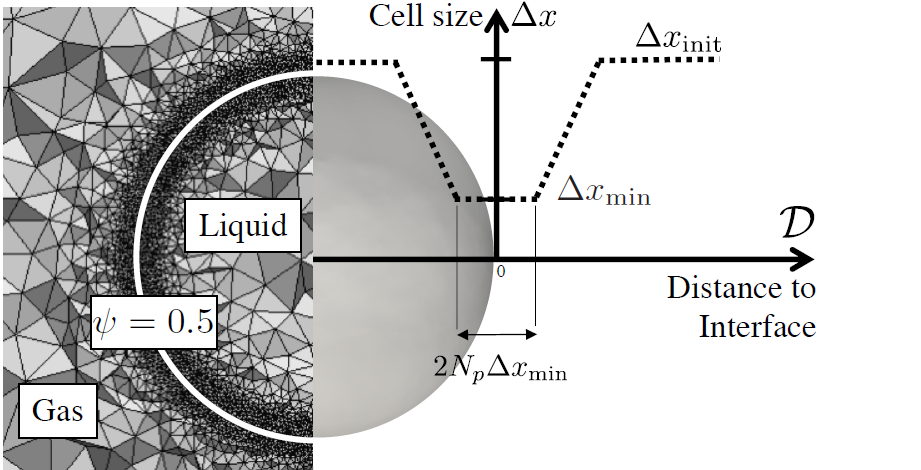
\includegraphics[width=0.6\textwidth]{./part1_numerical_approaches/figures_ch2/AMR}
       \centering
    \caption{Illustration of dynamic mesh adaptation with Adaptive Mesh Refinement. Source: \citepColor[leparoux_primary_2018].}
    \label{fig:AMR_strategy}
\end{figure}


